\documentclass{ctexart}
\usepackage[a4paper,total={6in,8in}]{geometry}
\usepackage{fancyhdr}
\usepackage[table,xcdraw]{xcolor}
\usepackage[utf8]{inputenc}
\usepackage{ctex}
\usepackage{color}
\usepackage{subfigure}
\usepackage{cite}
\usepackage{graphicx}
\usepackage{fontspec}
\setmainfont{Times New Roman}
\newfontfamily\timesfont{Times New Roman}
\usepackage{CJK}
\usepackage{indentfirst}
\usepackage{amsmath}
\usepackage{mathrsfs}
\usepackage{multirow}
\usepackage{svg}
\usepackage{amsfonts}
\usepackage{geometry}
\usepackage{hyperref}
\usepackage{mathabx}
\usepackage{cases}
\usepackage{minipage-marginpar}
\usepackage{xcolor}
% 导入包
\usepackage{hyperref}
% 格式设置
\hypersetup{hidelinks,
	colorlinks=true,
	allcolors=blue,
	pdfstartview=Fit,
	breaklinks=true}

\begin{document}

\begin{titlepage}
    \title{{\fontsize{28}{32}\selectfont\kaishu 机器人学 \\ \fontsize{20}{24}\selectfont\kaishu{作业5:运动学轨迹规划}}}
    \date{} % delete date as you want
    \maketitle
    \vspace{-7em}
    \begin{center}
      \fontsize{18}{22}\selectfont
      \textbf{\timesfont Robotics (2023-2024-2) \\
      Homework 5: Kinematic Trajectory Planning}
    \end{center}
    
    \begin{figure}[h]
        \centering
        
\includegraphics[width=0.45\textwidth]{Image/校标-校徽.png}
    \end{figure}
    \begin{center}
      \hspace{6em}
      \renewcommand{\arraystretch}{2}
      \begin{tabular}{rl}
      \fontsize{16}{50}\selectfont\heiti 姓名:& \fontsize{16}{24}\selectfont\heiti 赵四维 \\
      \fontsize{16}{24}\selectfont\heiti 学号:& \fontsize{16}{24}\selectfont 521021910696 \\
      \fontsize{16}{24}\selectfont\heiti 班级:& \fontsize{16}{24}\selectfont ME3403-01 \\
      \fontsize{16}{24}\selectfont\timesfont E-mail:& \fontsize{16}{24}\selectfont racheus.11@sjtu.edu.cn \\
      \end{tabular}
    \end{center}
    \begin{center}
      \fontsize{16}{24}\selectfont\timesfont \today
    \end{center}
\end{titlepage}

\pagenumbering{arabic}

\newpage
% \tableofcontents


\newpage
\pagestyle{fancy}
\fancyhf{}
\fancyhead[L]{ME3403-01}
\fancyhead[C]{机器人学Homework1}
\fancyhead[R]{赵四维 521021910696}
\fancyfoot[C]{\thepage}
\section{2R机械臂的运动学分析}
\subsection{Jacobian Matrix}
[Solution]:\par

根据题目要求,我们需要求解2R机械臂的雅可比矩阵。首先我们需要求解机械臂的正运动学方程,即末端执行器的位置和姿态与关节角度的关系。根据题目给出的机械臂结构,我们可以得到机械臂的正运动学方程如下:

\begin{equation}
	\left \{\begin{array}{c}
		x = l_1 \cos(\theta_1) + l_2 \cos(\theta_1 + \theta_2) \\
		y = l_1 \sin(\theta_1) + l_2 \sin(\theta_1 + \theta_2) \\
		\phi = \theta_1 + \theta_2		
	\end{array} \right.
\end{equation}

其中,$x, y, \phi$分别代表末端执行器的位置和姿态,$\theta_1, \theta_2$分别代表机械臂的两个关节角度,$l_1, l_2$分别代表机械臂的两个连杆长度。根据正运动学方程,通过求导可以求解出机械臂的雅可比矩阵如下:
\begin{equation}
	\left\{\begin{array}{c}
		\dot{x} = -l_1 \sin(\theta_1) \dot{\theta_1} - l_2 (\dot{\theta_1} + \dot{\theta_2}) \sin(\theta_1 + \theta_2)  \\
		\dot{y} = l_1 \cos(\theta_1) \dot{\theta_1} + l_2  (\dot{\theta_1} + \dot{\theta_2}) \cos(\theta_1 + \theta_2)  \\
		\dot{\phi} = \dot{\theta_1} + \dot{\theta_2}
	\end{array}\right.
\end{equation}

由$[\dot{x}, \dot{y}, \dot{\phi}]^T = J \cdot [\dot{\theta_1}, \dot{\theta_2}]^T$,我们可以得到雅可比矩阵$J$如下:

\begin{equation}
	J = \begin{bmatrix}
		\frac{\partial x}{\partial \theta_1} & \frac{\partial x}{\partial \theta_2} \\
		\frac{\partial y}{\partial \theta_1} & \frac{\partial y}{\partial \theta_2} \\
		\frac{\partial \phi}{\partial \theta_1} & \frac{\partial \phi}{\partial \theta_2}
	\end{bmatrix} = \begin{bmatrix}
		-l_1 \sin(\theta_1) - l_2 \sin(\theta_1 + \theta_2) & -l_2 \sin(\theta_1 + \theta_2) \\
		l_1 \cos(\theta_1) + l_2 \cos(\theta_1 + \theta_2) & l_2 \cos(\theta_1 + \theta_2) \\
		1 & 1
	\end{bmatrix}
\end{equation}

由《线性代数》课程知识,我们可以讨论Jacobian矩阵的秩。将矩阵的第二列的$(-1)$倍加到第一列,我们可以得到如下的矩阵:
\begin{equation}
	J = \begin{bmatrix}
		-l_1 \sin(\theta_1) - l_2 \sin(\theta_1 + \theta_2) & -l_2 \sin(\theta_1+\theta_2) \\
		l_1 \cos(\theta_1) + l_2 \cos(\theta_1 + \theta_2) & l_2 \cos(\theta_1+\theta_2) \\
		1 & 1
	\end{bmatrix}
	\stackrel{\text{$-r_2+r_1$}}{\longrightarrow}
	\begin{bmatrix}
		-l_1 \sin(\theta_1) & -l_2\sin(\theta_1+\theta_2)\\
		l_1  \cos(\theta_1) &l_2 \cos(\theta_1+\theta_2) \\
		0 & 1\\
	\end{bmatrix}
\end{equation}

从数学角度看,如果Jacobian矩阵的秩为1,需要满足如下的条件:
\begin{equation}
	\left\{\begin{array}{c}
		-l_1 \sin(\theta_1) = 0 \\
		l_1 \cos(\theta_1) = 0
	\end{array}\right.
\end{equation}

且二者需要同时满足。由正余弦函数的相位差可知,两个条件总是不能\textbf{同时满足}的。因此,我们可以Jacobian矩阵的秩为2。这一点也可以从机械原理上得到印证,因为机械臂的自由度是由关节的个数决定的,而2R机械臂的自由度为2,这一点是相互印证的。

[Appendix]笔者个人理解,题目中的Jacobian矩阵和我们常规定义的Jacobian矩阵有一定的区别。常规定义的Jacobian矩阵是2*2的矩阵,形如:
\begin{equation}
	J = \begin{bmatrix}
		\frac{\partial x}{\partial \theta_1} & \frac{\partial x}{\partial \theta_2} \\
		\frac{\partial y}{\partial \theta_1} & \frac{\partial y}{\partial \theta_2}
	\end{bmatrix}
	= \begin{bmatrix}
		-l_1 \sin(\theta_1) - l_2 \sin(\theta_1 + \theta_2) & -l_2 \sin(\theta_1 + \theta_2) \\
		l_1 \cos(\theta_1) + l_2 \cos(\theta_1 + \theta_2) & l_2 \cos(\theta_1 + \theta_2)
	\end{bmatrix}
\end{equation}

这种情况下,取特殊情况$\theta_1 = \theta_2 = 0$,我们可以得到:
\begin{equation}
	J_{0} = \begin{bmatrix}
		0 & 0 \\
		l_1+l_2 & l_2
	\end{bmatrix}
\end{equation}

在这种情况下存在0行,因此Jacobian矩阵的秩为1。但是相同的特殊情况作用于题目中的3*2矩阵,我们可以得到:
\begin{equation}
	J_{0}^\prime = \begin{bmatrix}
		0 & 0 \\
		l_1+l_2 & l_2 \\
		1 & 1
	\end{bmatrix}
\end{equation}

显然,在这种特殊情况下,上述(8)矩阵中$l_1+l_2 \neq l_2$,因此Jacobian矩阵的秩为2。所以本题中的Jacobian矩阵的秩一定为2。

\subsection{MATLAB Operation}
\href{src/Rhw1_2_main.m}{Click here to jump to the MATLAB code.}

第二问是第一问的延续,只需在MATLAB中编辑相应的矩阵即可,这里不再赘述。

输入为两个关节角度(弧度制),终端输出Jacobian矩阵,并在窗口中画出对应的机械臂姿态。

[demo:]
\begin{figure}[h]
	\centering
	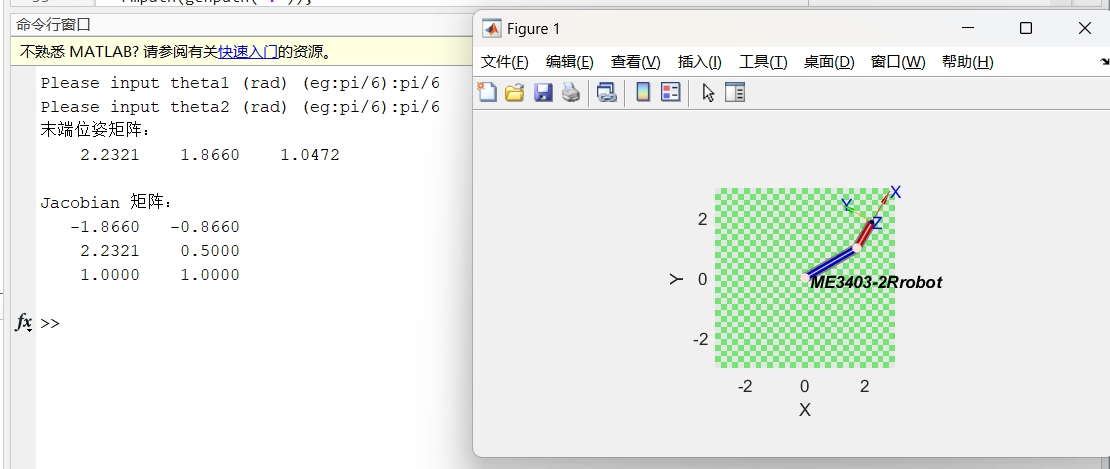
\includegraphics[width=0.8\textwidth]{Image/2.png}
	\caption{$[\pi/6,\pi/6]$对应的机械臂的姿态}
\end{figure}

\subsection{MATLAB Kinematics Inverse Solution}
\href{src/Rhw1_3_main.m}{Click here to jump to the MATLAB code.}

\begin{figure}[h]
	\centering
	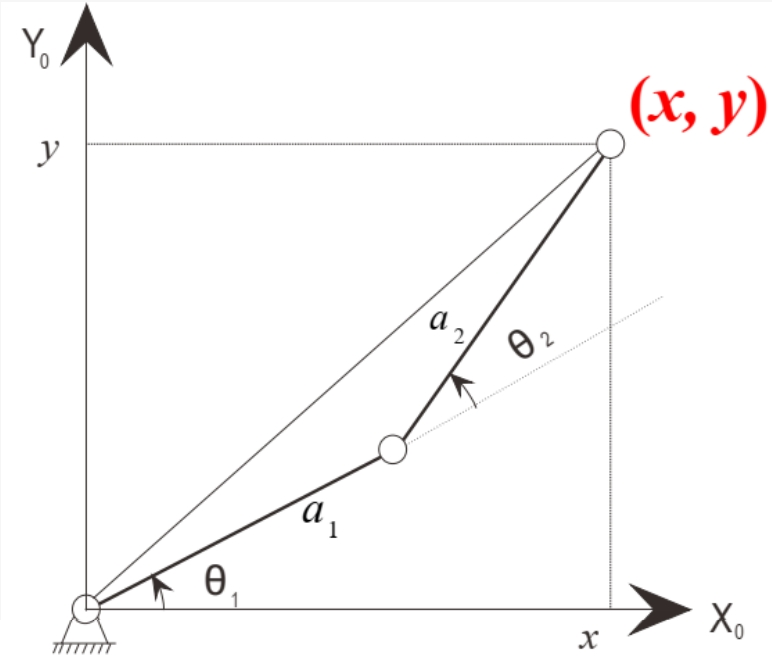
\includegraphics[width=0.4\textwidth]{Image/formula.png}
	\caption{任一时刻的姿态}
\end{figure}

易得:

$$D=\cos \theta_2 = \frac{x^2+y^2-a_1^2-a_2^2}{2a_1a_2}$$
$$\theta_2 = \arctan2(\frac{\sqrt{1-D^2}}{D})$$
$$\theta_1 = \arctan2(y,x) - \arctan2(a_2\sin\theta_2,a_1+a_2\cos\theta_2)$$

需要注意,这里的$\arctan2$函数是MATLAB中的atan2函数,这个函数在机器人学中至关重要,其优势在于可以正确地处理四个象限的所有角度,并且避免了由于除数为零而产生的错误,它的定义为:

$$\arctan2(y,x) = \begin{cases}
	\arctan(\frac{y}{x}) & x>0 \\
	\arctan(\frac{y}{x})+\pi & x<0,y\geq 0 \\
	\arctan(\frac{y}{x})-\pi & x<0,y<0 \\
	\frac{\pi}{2} & x=0,y>0 \\
	-\frac{\pi}{2} & x=0,y<0 \\
	\text{undefined} & x=0,y=0		
\end{cases}$$															

第三问重点在于数学公式的推导和求解的判断。但是需要注意解的存在性。比如给定矩阵$p=[2.5\quad 2.5\quad \frac{\pi}{6}]^T$,在这个位置上显然通过集合求解会有两个值,但是两个值末端的姿态角均不满足$\theta_1+\theta_2=\frac{\pi}{6}$要求。因此,我们需要对解的存在性进行判断。
\newpage

[demo:]
\begin{figure}[h]
	\centering
	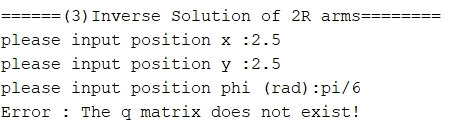
\includegraphics[width=0.7\textwidth]{Image/3.png}
	\caption{任一时刻的姿态}
\end{figure}

\subsection{Trajectory Planning}
\href{src/Rhw1_4_main.m}{Click here to jump to the MATLAB code.}

直接点击运行即可。

绘制轨迹如图:

\begin{figure}[h]
	\centering
	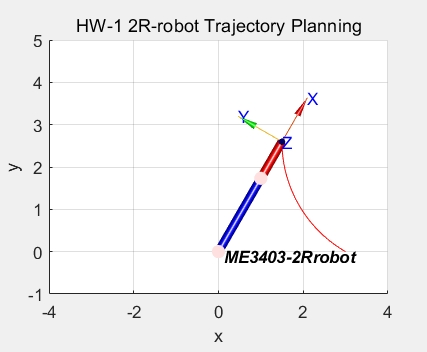
\includegraphics[width=0.6\textwidth]{Image/trajectory.png}
	\caption{任一时刻的姿态}
\end{figure}

运动轨迹视频:
\href{src/robot_trajectory.avi}{Click here to jump to the video.}

本作业汇报使用\LaTeX 编写,秉持着\textbf{记录学习与成长、资源开放和共享}之精神,笔者也将源代码已经上传至\href{https://github.com/Racheus/Robotics-Caprice/tree/master/Homework1-2Rrobot-Kine}{here}。
如果有前面作业有无法打开或者链接错误等情况,烦请助教老师在上面这个链接里查看作业源代码。当然出于研究兴趣,笔者写了一个第四题的Python版本,尝试不调用前辈的库自己绘图,附在上述链接中。


\end{document}